\documentclass{article}
\usepackage[italian]{babel}
\usepackage[utf8]{inputenc}
\usepackage{fancyhdr}
\usepackage{tikz}
\usepackage{amsmath}
\usepackage{amssymb}
\usepackage{amsthm}
\usepackage{amsfonts}
\usepackage{color}
\usepackage{circuitikz}
\usepackage[margin=2cm]{geometry}
\usepackage[scientific-notation=true]{siunitx}
\usepackage{titlesec}
\usepackage{graphics}

\titleformat{\paragraph}
  {\normalfont\normalsize\bfseries}{\theparagraph}{1em}{}
\titlespacing*{\paragraph}
  {0pt}{3.25ex plus 1ex minus .2ex}{1.5ex plus .2ex}

\title{Analisi di un circuito RLC serie in regime sinusoidale}
\date{18/05/2022}
\author{Bertasi Leonardo mat. 970881, Perniola Davide mat. 989409}
\begin{document}
\maketitle
\section{Abstract} 
In questa esperienza si è analizzato il comportamento di un circuito RLC in regime sinusoidale. Misurando le tensioni ai capi delle componenti è stato possibile
verificare la differenza di comportamento del circuito il un ampio range di frequenze intorno alla frequenza di risonanza attesa $f_0=(7351\pm68)Hz$...
Inoltre si è studiato l'andamento dell'ampiezza e della fase delle tensioni ai capi delle componenti in funzione della frequenza


\section{Introduzione} 
Un circuito RLC serie consiste in una resistenza, una induttanza e un condensatore posti in serie. Applicando ai capi del ciruito una differenza di potenziale sinusoidale $V_{0}\cos{wt} $ ci si aspetta di osservare un preciso andamento, anch'esso sinusoidale,
 ai capi di ognuno degli elementi circuitali. L'unica corrente che scorre nel circuito segue la relazione(si veda appendice) 
\begin{equation}
  i(t)=\frac{V_{0}}{\sqrt{R^2+(wL-\frac{1}{wC})^2}}\cos{[wt+(\arctan{\frac{1-w^2LC}{wRC}})]}
\end{equation}
Utilizzando la (1) si possono scrivere gli andamenti teorici della ddp ai capi della resistenza
\begin{equation}
 V_{R}(t)= \frac{V_{0}R}{\sqrt{R^2+(wL-\frac{1}{wC})^2}}\cos{[wt+(\arctan{\frac{1-w^2LC}{wRC}})]}
\end{equation}

dell'induttanza
\begin{equation}
  V_{L}(t)=\frac{V_{0}wL}{\sqrt{R^2+(wL-\frac{1}{wC})^2}}\cos{[wt+(\arctan{\frac{1-w^2LC}{wRC}})+\frac{\pi}{2}]}
\end{equation}
e del condensatore
\begin{equation}
  V_{C}(t)=\frac{(\frac{V_{0}}{wC})}{\sqrt{R^2+(wL-\frac{1}{wC})^2}}\cos{[wt+(\arctan{\frac{1-w^2LC}{wRC}})-\frac{\pi}{2}]}
\end{equation} 

Ricordando che la pulsazione di risonanza per un circuito RLC è $w_0=\frac{1}{\sqrt{LC}}$ e che il modulo della corrente che scorre nel circuito alla frequenza di risonanza corrispondente $f_0$ è massimo, alla frequenza di risonanza ci si aspetta di 
osservare $V_R(t)$ in fase con la sorgente e massimo in ampiezza, $V_L(t)$ in anticipo di $\frac{\pi}{2}$ rispetto alla sorgente e $V_C(t)$ in ritardo di $\frac{\pi}{2}$ rispetto alla sorgente e della stessa ampiezza di  $V_C(t)$. Inoltre ci 
si aspetta, aumentando $w$, una diminuzione dell'ampiezza di $V_R(t)$ a seguito del massimo in $w_0$, un aumento dell'ampiezza di  $V_L(t)$
e una diminuzione dell'ampiezza di $V_C(t)$. Per quanto riguarda la fase inoltre, notando come 
\begin{equation}
  \lim_{w \to + \infty}\arctan{\frac{1-w^2LC}{wRC}} = -\frac{\pi}{2}
\end{equation}
è chiaro aspettarsi, aumentando $w$, la decrescita della fase della ddp ai capi di ogni componente e lo stabilizzarsi di quest'ultima a $-\frac{\pi}{2}$ per $V_R(t)$, 0 per $V_L(t)$ e $-\pi$ per $V_C(t)$.





\section{Apparato sperimentale e svolgimento}
\begin{figure}[h!]
  \begin{center}
    \begin{circuitikz}[]
      \draw (0,0)
      to[vsourcesin=$V_S$] (0,2) % The voltage source
      to[R=$R_I$] (0,4)
      

      to[R=$R$] (2,4) % The resistor
      to[R=$R_L$] (4,4)
      
      to[L=$L$] (4,0)
      to[short] (4,0)
      to[C=$C$] (0,0)
      to[short] (0,0);

    \end{circuitikz}
    \caption{\textit{Schema del circuito realizzato.}}
  \end{center}
\end{figure}
Il circuito RLC è stato realizzato sulla breadboard della scheda di acquisizione NI ELVIS II ed è schematizzato in Figura 1. Esso è alimentato dal function generator di ELVIS di resistenza interna $R_I=50\Omega$ come da specifiche della scheda. Nel ciruito sono presenti, disposti in serie, 
una induttanza $L=(10.3\pm0.1)mH$, un condensatore $C=(45.5\pm0.4)nF$ una resistenza $R=(330.0\pm0.3)\Omega$ e una resistenza $R_L=(34.5\pm0.1)\Omega$ che tiene conto della resistenza interna dell'induttore. Tutti i valori delle componenti riportati sono stati misurati utilizzando il multimetro digitale di ELVIS.
Per verificare il corretto funzionamento delle componenti è stato utilizzato un oscilloscopio, osservando così il comportamento del ciruito in un intorno della frequenza di risonanza attesa. Successivamente servendosi di un programma scritto in LabView sono state acquisite le misure delle ddp ai capi del generatore, resistenza, induttanza e consensatore relative ad una frequenza $f_m=4000Hz$, una $f_0=7351Hz$ e  $f_M=10000Hz$ in modo tale da evidenziare le differenze del comportamento del circuito all'interno di un ampio range di frequenze e in particolare alla frequenza di risonanza.
Per far questo si è usata una frequenza di acquisizione di $\SI{5e4 }Hz$ nel primo caso, di $\SI{1e5 }Hz$ nel secondo e di $\SI{1.5e5 }Hz$ nel terzo, affinchè questa si mantenga ad un valore di almeno dieci volte quello della frquenza del segnale acquisito.
Infine si è studiato l'andamento della fase e dell'ampiezza della ddp ai capi delle componenti in funzione della frequenza. Per far ciò si è impostato nel funcion generetor uno \textit{sweep} sulla frequenza nel range compreso tra $3000Hz$ e $13000Hz$, con \textit{step} di $100 Hz$ e \textit{step interval} di $100 ms$. 

\section{Risultati e discussione}
\subsection{Tensione in funzione del tempo}
\begin{figure}[]
  \centering
  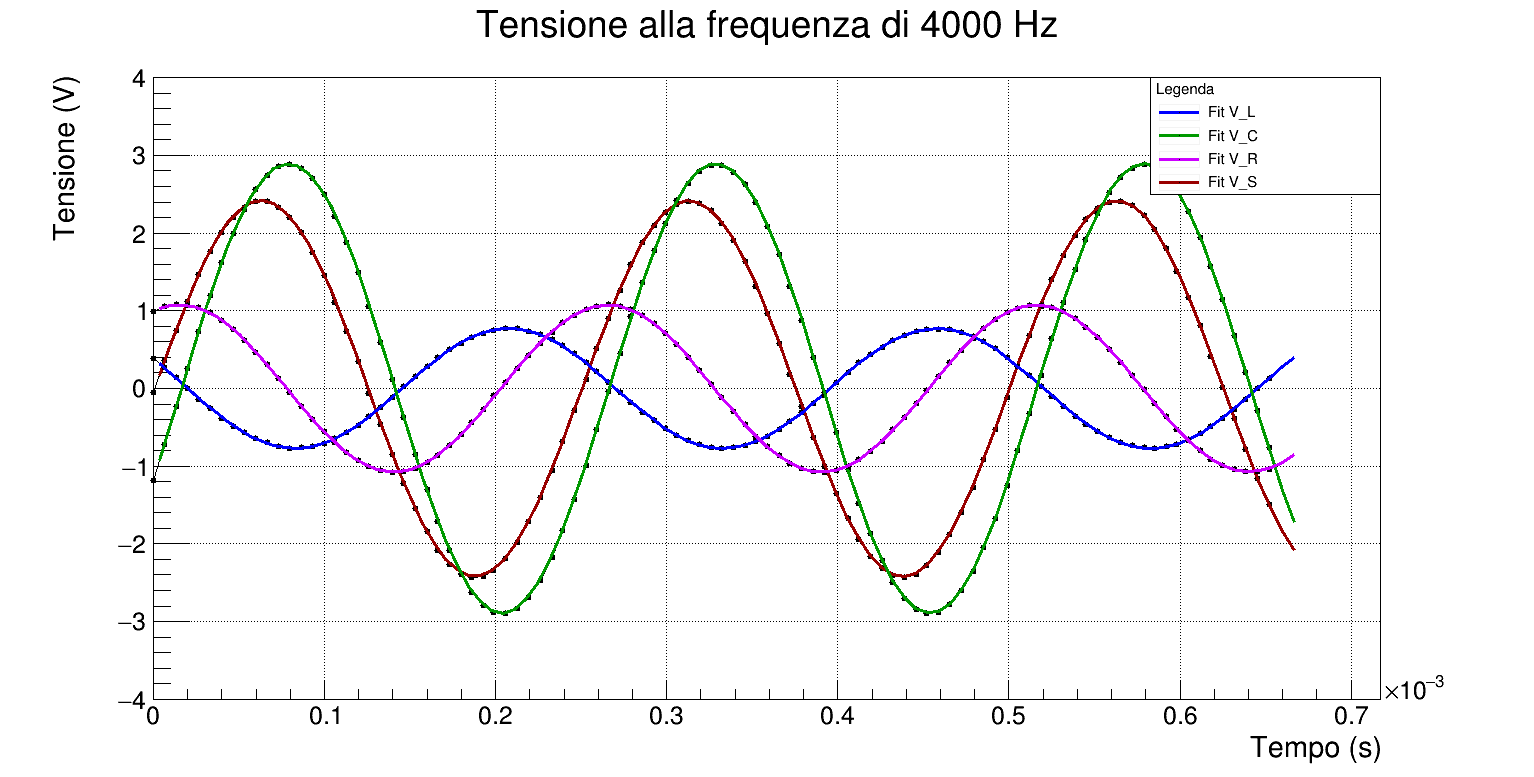
\includegraphics[scale=0.27]{FitFMin.png}
  \qquad
  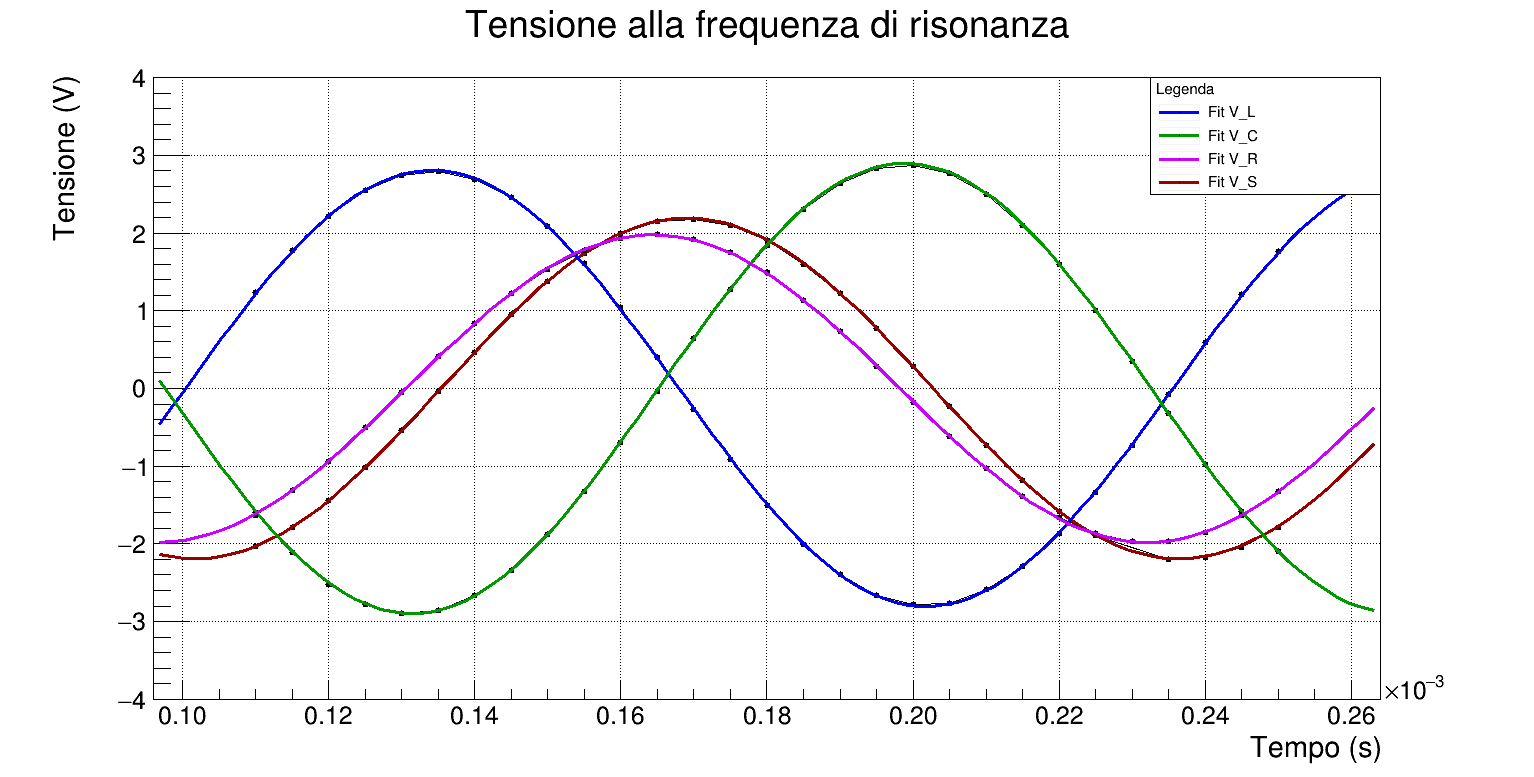
\includegraphics[scale=0.27]{FitF0.png}
  \qquad
  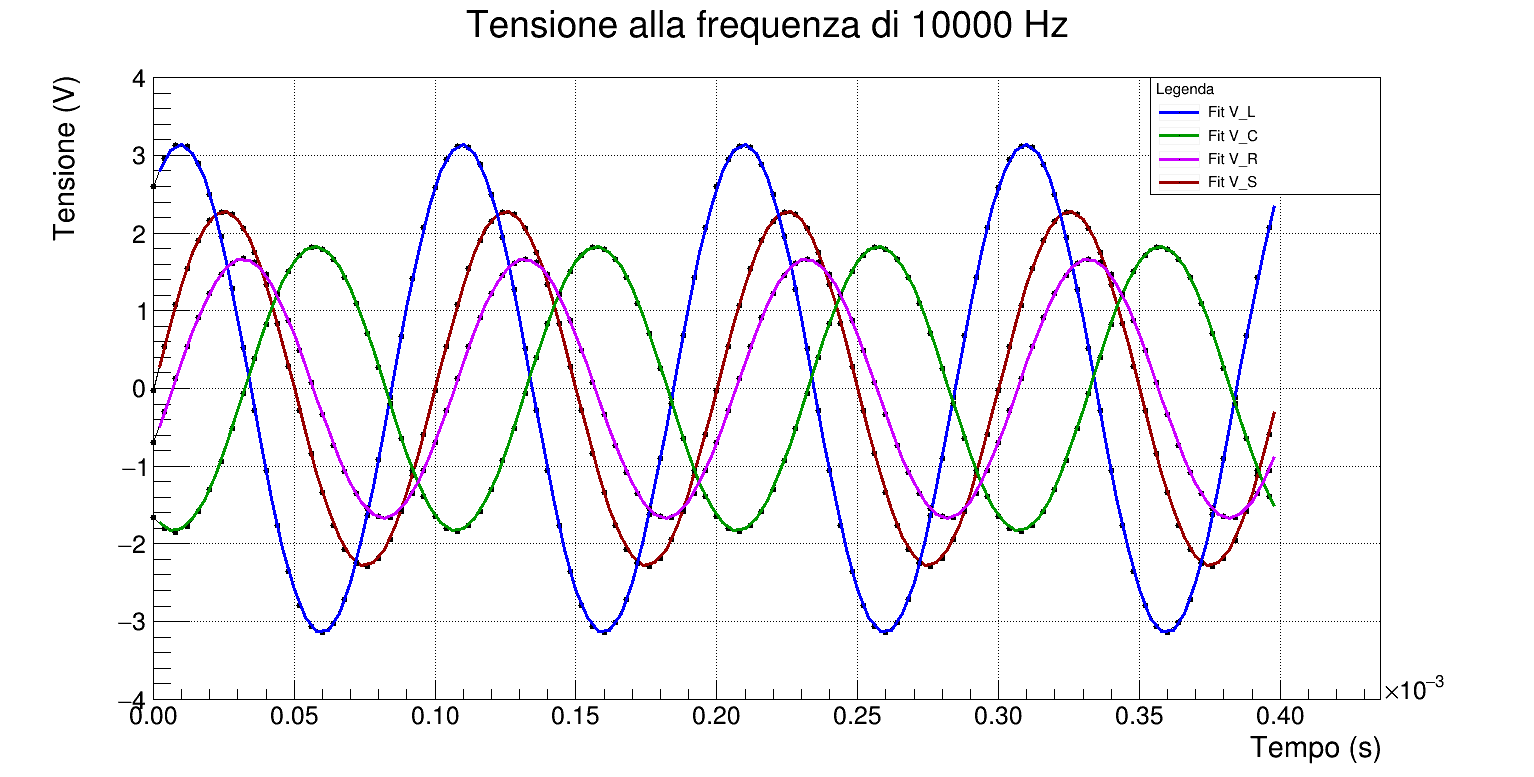
\includegraphics[scale=0.27]{FitFMag.png}
  \caption{\textit{Confronto tra le tensioni in funzione del tempo ai capi degli elementi circuitali relativi alle tre diverse frequenze utilizzate. In alto $f_m$,in mezzo $f_0$ e in basso $f_M$ .}}
\end{figure}
In Figura 2 sono riportate le tensioni in funzione del tempo ai capi di ogni elemento del circuito per valori minori uguali e maggiori alla frequenza di risonanza. 
In Figura 2 sono riportate le tensioni in funzione del tempo ai capi di ogni elemento del circuito per valori minori uguali e maggiori alla frequenza di risonanza. 
In Figura 2 sono riportate le tensioni in funzione del tempo ai capi di ogni elemento del circuito per valori minori uguali e maggiori alla frequenza di risonanza. 
In Figura 2 sono riportate le tensioni in funzione del tempo ai capi di ogni elemento del circuito per valori minori uguali e maggiori alla frequenza di risonanza. 
In Figura 2 sono riportate le tensioni in funzione del tempo ai capi di ogni elemento del circuito per valori minori uguali e maggiori alla frequenza di risonanza. 
In Figura 2 sono riportate le tensioni in funzione del tempo ai capi di ogni elemento del circuito per valori minori uguali e maggiori alla frequenza di risonanza. 

\subsection{Analisi dell'ampiezza}
\begin{figure}
  \centering
  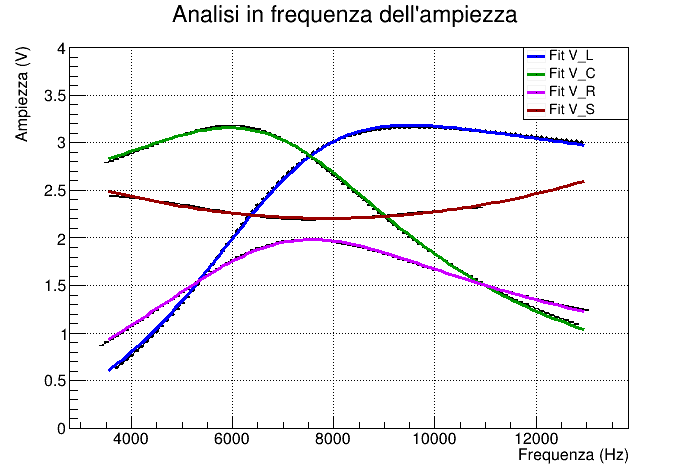
\includegraphics[scale=0.4]{AmpFreq.png}
\end{figure}
\subsection{Analisi della fase}
\begin{figure}
  \centering
  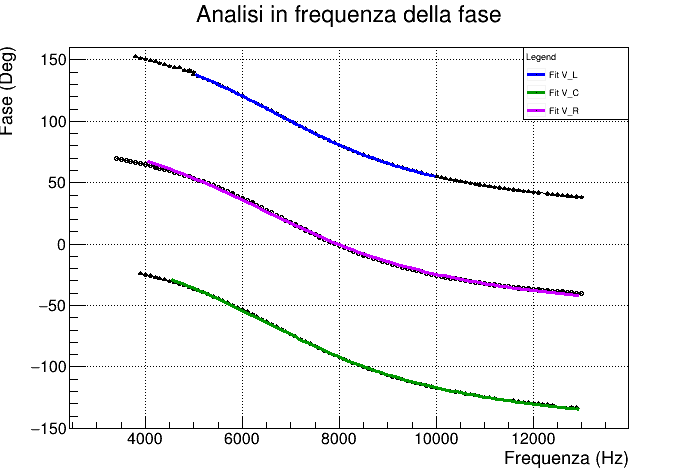
\includegraphics[scale=0.4]{FaseFreq.png}
\end{figure}
\section{Conclusioni}
\section{Appendice}
\begin{itemize}
  \item Per ricavare la (1) è necessario risolvere l'equazione differenziale lineare al secondo ordine
$$
L\frac{dI}{dt}+RI+\frac{1}{C}\int{Idt}=V_0\cos{wt}
$$  
  
\end{itemize}
\end{document}
